\section{SAASFEE}
\label{saasfee}

%one page, should include an evaluation (see Introduction)
%one paragraph on saasfee (possibly w/ img)
%one paragraph on hiway
%one paragraph on cuneiform
%one paragraph on evaluation (w/ image)
% \vspace{-5mm}

To process the vast amounts of genomic data stored in today's Biobanks, researchers have a diverse ecosystem of tools at their disposal~\cite{Pabinger2014}. Depending on the research question at hand, these tools are often used in conjunction with one another, resulting in complex and intertwined analysis pipelines. Scientific workflow management systems (SWfMSs) facilitate the design, refinement, execution, monitoring, sharing, and maintenance of such analysis pipelines. SAASFEE~\cite{vldb_demo} is a SWfMS that supports the scalable execution of arbitrarily complex workflows. It encompasses the functional workflow language Cuneiform as well as Hi-WAY, a higher-level scheduler for both Hadoop YARN and HopsYARN.

Analysis pipelines for large-scale genomic data employ many different software tools and libraries with diverse Application Programming Interfaces (APIs). At the same time the growing amounts of data to be analyzed necessitate parallel and distributed execution of these analysis pipelines. Thus, the methods for specifying such analysis pipelines need to meet both concerns -- integration and parallelism equally. The functional workflow Language Cuneiform has been designed to meet these requirements~\cite{Brandt2015}. Cuneiform allows the integration of software tools and libraries with APIs in many different programming languages. This way, command-line tools (e.g., Bowtie) can be integrated with similar ease as, for instance, R libraries (e.g., CummeRbund). By partitioning large data sets and processing these partitions in parallel, data parallelism can be exploited in addition to task parallelism to speed up computation. Cuneiform automatically detects and exploits data and task parallelism in a workflow specification. Editing and debugging workflows is supported by the tools and visualization features provided with the Cuneiform interpreter.

Hi-WAY provides a selection of established scheduling policies conducting task placement based on
\begin{inparaenum}[(a)]
  \item the locality of a task's input data to diminish network load and
  \item task runtime estimation based on past measurements to utilize resources efficiently.
\end{inparaenum}
To enable repeatability of experiments, Hi-WAY generates exhaustive provenance traces during workflow execution, which can be shared and re-executed or archived in a database. One of the major distinctive features of SAASFEE is its strong emphasis on integration of external software. This is true for both Cuneiform, which is able to integrate foreign code and command-line tools, and Hi-WAY, which is capable of running not only Cuneiform workflows, but also workflows designed in the SWfMSs Pegasus~\cite{pegasus_fgcs} and Galaxy~\cite{Goecks10}.

To verify the scaling behavior of SAASFEE for large-scale use cases relevant for Biobanks, we specified and ran a variant calling pipeline on 10~GB of compressed whole genome sequencing reads from the 1000 Genomes Project. These reads were aligned against a reference genome, variants were called, and the resulting sets of variants were annotated using publicly available databases. Figure~\ref{fig:saasfee_scaling} shows the scalability of this workflow. Within the limits of the setup chosen, linear scaling behavior could be achieved for the variant calling workflow.

\begin{figure}
  \centering
  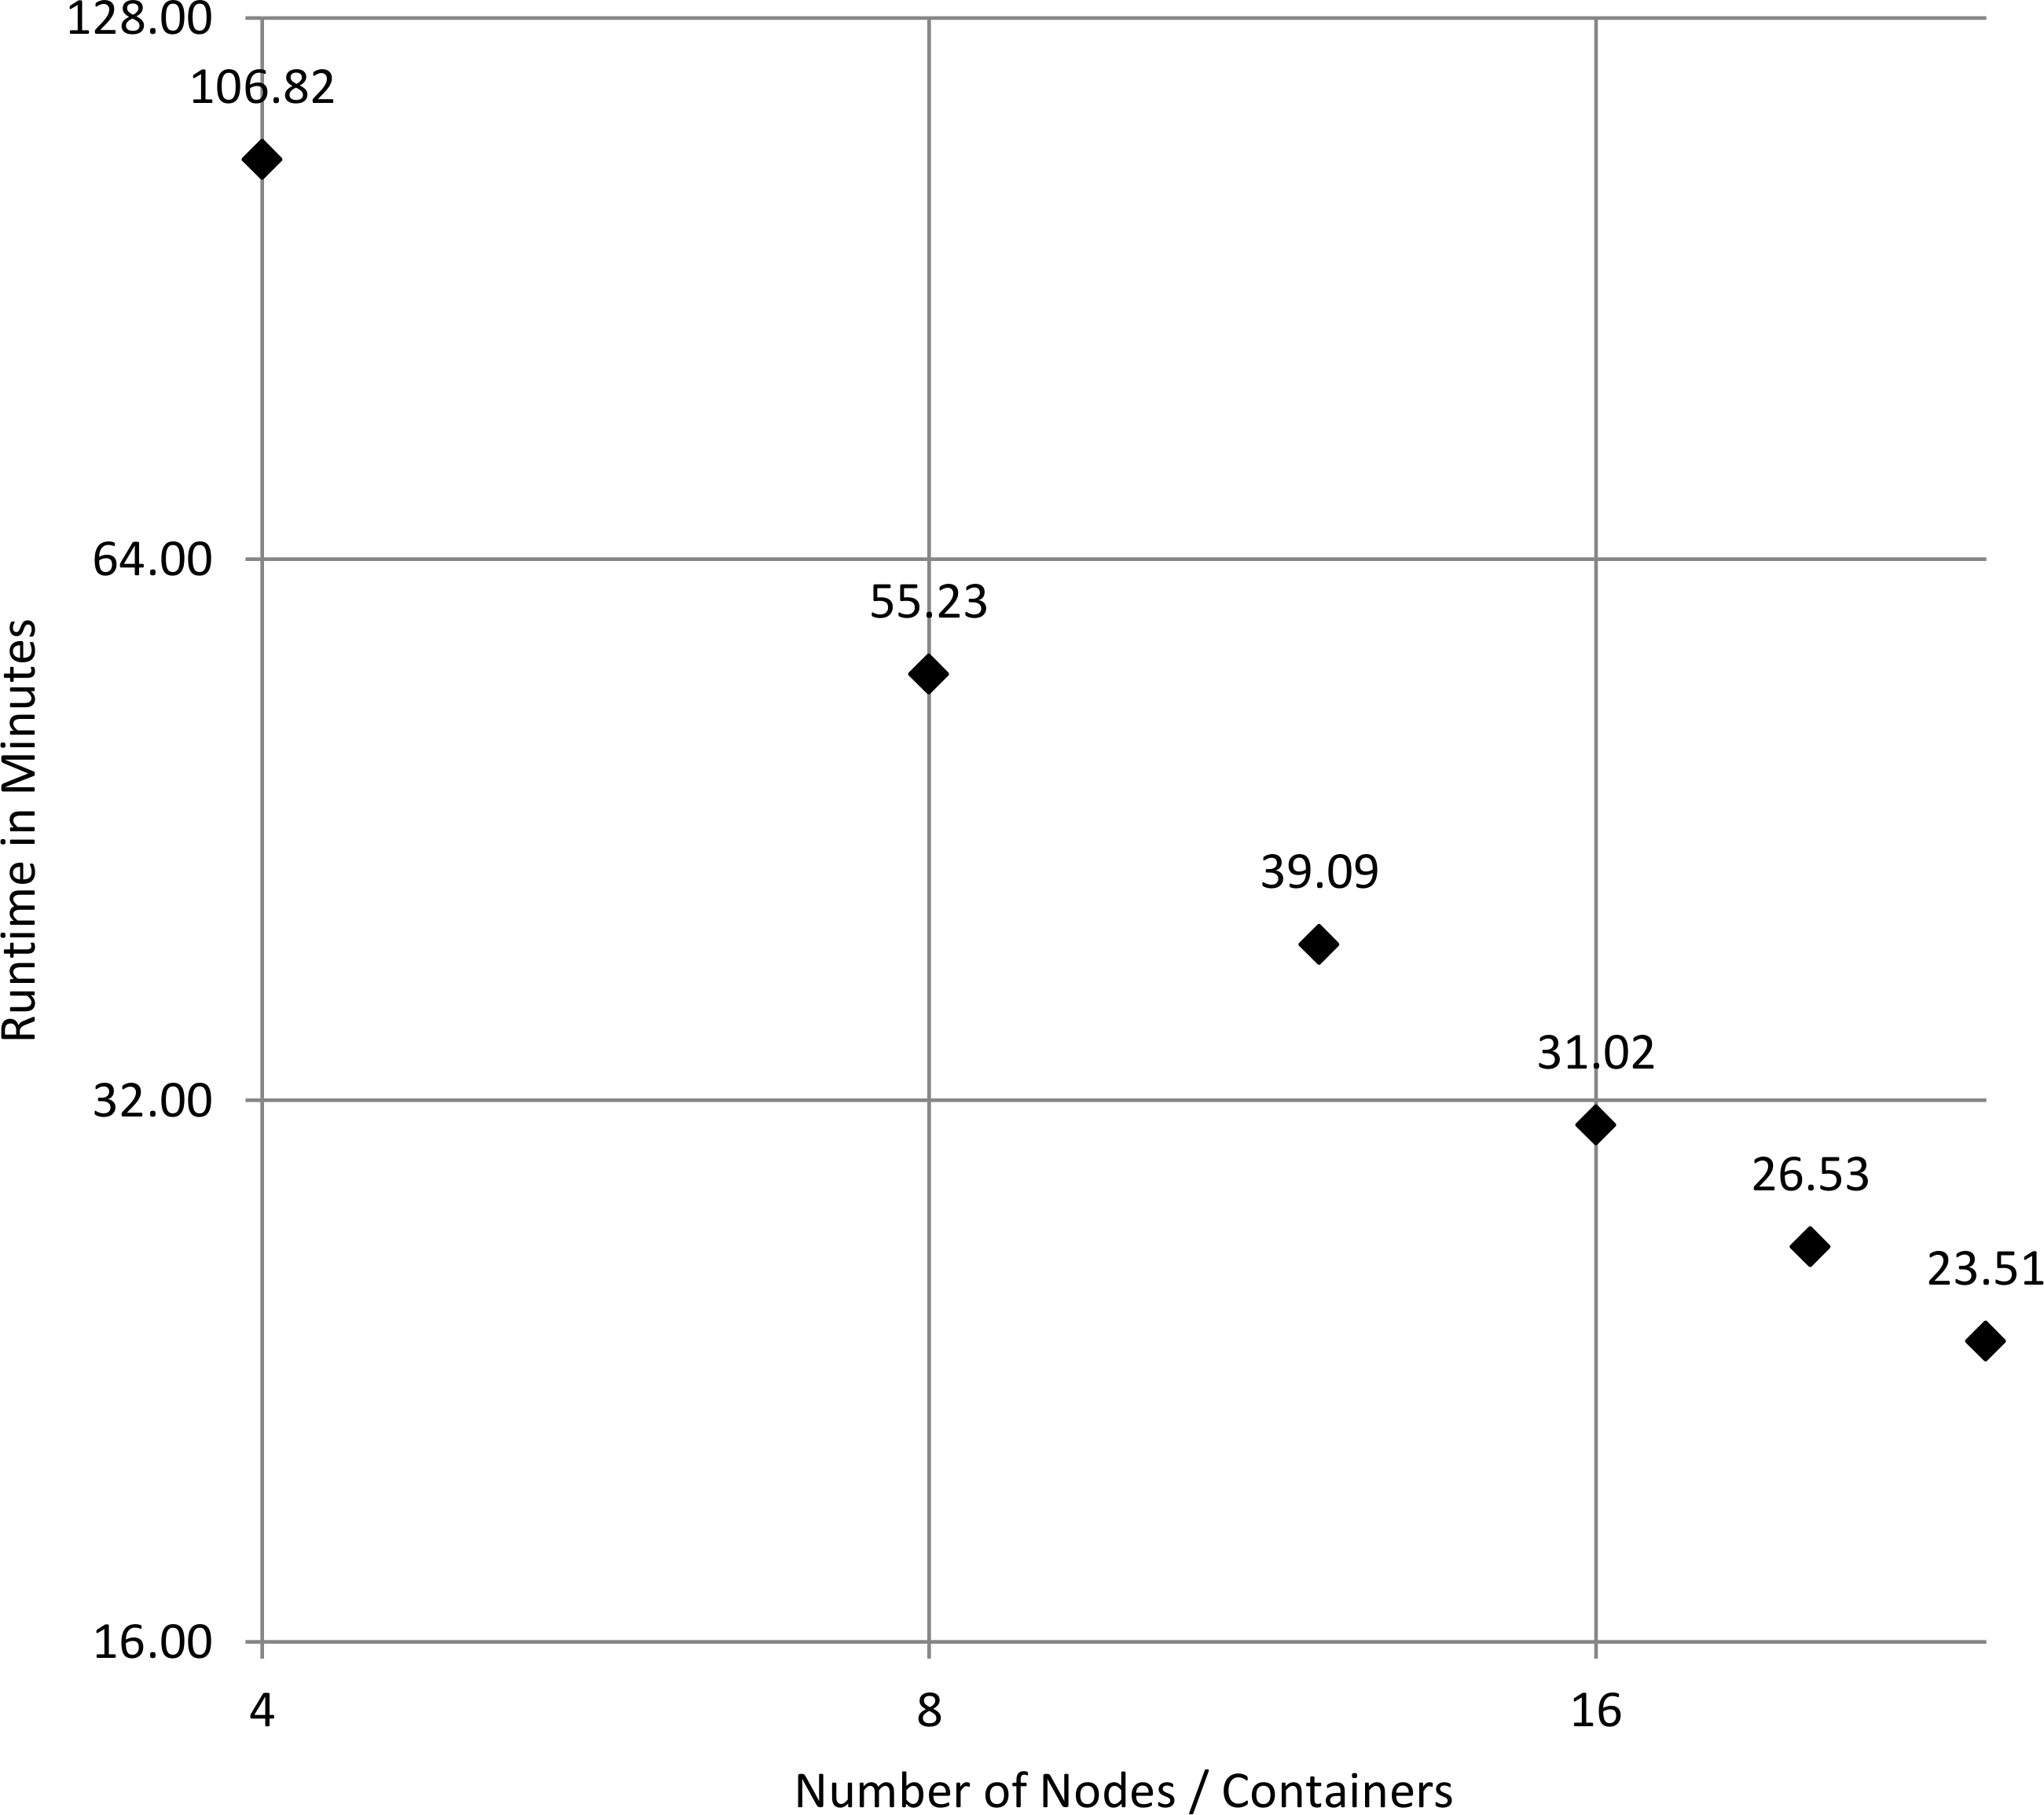
\includegraphics[width=.55\textwidth]{imgs/wf_runtime.png}
  \caption{Scalability experiment for the SAASFEE software stack. A variant calling workflow has been scaled out on up to 24 nodes. Both axes, the runtime in minutes and the number of nodes are on a logarithmic scale (published in Brandt et al. 2015~\cite{Brandt2015}).}
  \label{fig:saasfee_scaling}
\end{figure}
\vspace{-5mm}
